\section{Auswertung}
\label{sec:Auswertung}

\subsection{Die Aktivit"at der Americum-Quelle}
  Die Aktivit"at/Z"ahlrate $Z_{Quelle}$ der $^{241}\text{Am}$-Quelle wird gegeben druch
  \begin{equation}
    \frac{4\pi(\SI{0,041}{\meter}+\SI{0,039}{\meter}+\SI{0.017}{\meter})^2}{3F}Z_{gemessen}
  \end{equation}
  ,weil davon ausgegangen wird, dass die Quelle homogen in alle Raumrichtungen strahlt.
  Mit $Z_{gemessen}=\SI{13,5}{\becquerel}$ ergibt sich:
  \begin{equation}
    Z_{Quelle} = \SI{274}{\kilo \becquerel} \; .
  \end{equation}

  Der theoretisch zu erwartende Wert kann mithilfe des klassischen Zerfallsgesetzes berechnet werden:
  \begin{equation}
    Z_{Quelle} = Z_0\text{e}^{\frac{\ln(2)t}{\tau}} \approx \SI{318}{\kilo \becquerel}
  \end{equation}
  Dabei ist $\tau=432,2$ Jahre die Halbwertszeit und $Z_0=\SI{330}{\kilo \becquerel}$ \cite{Anleitung} die urspr"ungliche Aktivit"at.


\subsection{\texorpdfstring{Bestimmung der Foliendicke einer Goldfolie durch Energieverlustmessung der $\alpha$-Teilchen}{Bestimmung der Foliendicke einer Goldfolie durch Energieverlustmessung der alpha-Teilchen}}





\subsection{Vermessung des Rutherford-Streugesetzes}
  Die gemessenen Z"ahlraten $Z(\theta)$ und zugeh"origen Streuwinkel $\theta$ so wie der jeweils nach Formel (\ref{querschnitt}) berechnete differentielle Wirkungsquerschnitt $\text{d}\sigma/\text{d}\Omega(\theta)$ sind in Tabelle (\ref{tab:ruther}) dargestellt.
  Dabei sind
  \begin{align*}
    F &= \SI{20e-6}{\meter \squared} \\
  \end{align*}


  \begin{table}
  \centering
  \begin{tabular}{c|c|c}

  Streuwinkel $\theta$ /Grad	&	Z"ahlrate $Z(\theta)/\frac{1}{\SI{60}{\second}}$	& $\frac{\text{d}\sigma}{\text{d}\Omega(\theta)}/\si{\meter \squared}$	 \\

  \toprule
 	0	   & 776 & 4.47e-21 \\
 	0,2	 & 662 & 3.82e-21 \\
 	0,4	 & 669 & 3.86e-21 \\
 	0,6	 & 583 & 3.36e-21 \\
  0,8  & 586 & 3.38e-21 \\
  1    & 612 & 3.53e-21 \\
  1,2  & 630 & 3.63e-21 \\
  1,4  & 635 & 3.66e-21 \\
  1,6  & 604 & 3.48e-21 \\
  1,8  & 642 & 3.70e-21 \\
  2    & 633 & 3.70e-21 \\
  2,2  & 615 & 3.55e-21 \\
  2,4  & 549 & 3.42e-21 \\
  2,6  & 621 & 3.58e-21 \\
  2,8  & 616 & 3.55e-21 \\
  3    & 634 & 3.66e-21 \\
  7    & 424 & 2.45e-21 \\
  10   & 260 & 1.50e-21 \\
  15   & 85  & 4.99e-22 \\
  20   & 26  & 1.52e-22 \\
 %\midrule

  %\multicolumn{2}{c}{$\overline{n}$} & \multicolumn{2}{c} {1,56 $\pm$ 0,02} \\
 \bottomrule
  \end{tabular}
  \caption{Streuwinkel und zugeh"orige Z"ahlrate so wie differentieller Wirkungsquerschnitt f"ur die $\SI{2}{\micro \meter}$-Goldfolie.}
  \label{tab:ruther}
  \end{table}


  Die experimentellen Werte ($\theta,\frac{\text{d}\sigma}{\text{d}\Omega(\theta)}$) sind zusammen mit der Theoriekurve nach (\ref{ruther}) in Abb. (\ref{plot:ruther}) aufgetragen.

  \begin{figure}
    \centering
    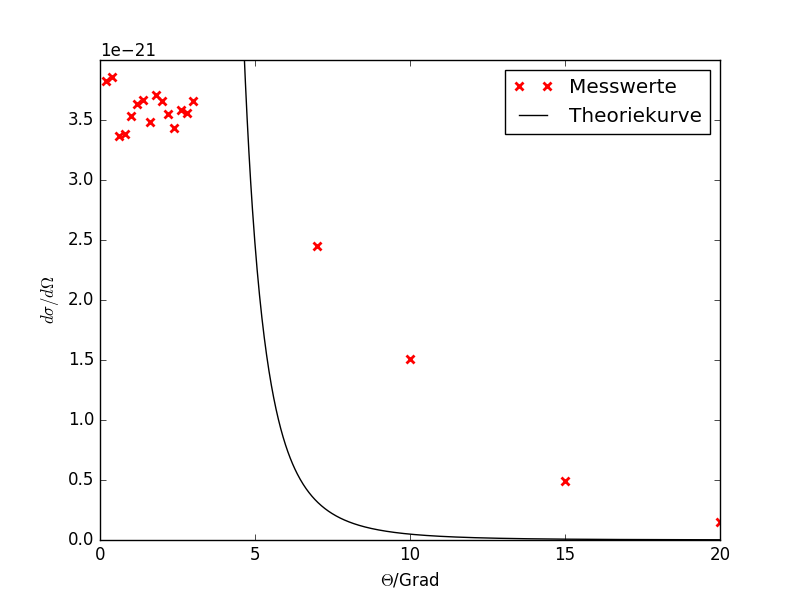
\includegraphics[width=15cm]{skripte/ruther.png}
    \caption{Messwerte und Theoriekurve f"ur das Rutherford-Streugesetz bei der $\SI{2}{\micro \meter}$-Goldfolie.}
    \label{plot:ruther}
  \end{figure}

  Wie zu erkennen ist, zeigen die Messwerte neben dem insgesamt abfallendem Trend keine gute "Ubereinstimmung mit der Theoriekurve.

  \newpage



  \subsection{Nachweis von Mehrfachstreuungen und und $Z$-Abh"angigkeit der Rutherford-Streuformel}
